\begin{frame}
  \begin{center}
    {\huge GloVe: Global Vectors for Word Representation
    }
    Pennington,Socher,Manning
  \end{center}
\end{frame}
%%%%%%%%%%%%%%%%%%%%%%%%%%%%%%%%%%%%%%%%%%%%%%%%%%

\begin{frame}{A Brief History of Word Vectors}
  %% Word vectors capture linguistic regularities in a simple manner.
  \begin{align*}
    king - man + woman \approx queen
  \end{align*}
  Ways to obtain word vectors:
  \begin{itemize}
  \item Compute Global Statistics (LSA etc.)
  \item Learn from Local Context (word2vec)
  \end{itemize}
  %% No explanation was given in the original papers.
  \footnotesize{Remarkably, training such a lexical model induces word repr. with striking semantic and syntactic properties.}---\cite{Mikolov13a} \\
  %% Levy showed that tranditional methods like count sparse contexts can perform equally well.
  \footnotesize{... traditional word similarities can perform just as well as neural embeddings.}---\cite{Levy14}
\end{frame}

\begin{frame}{Evaluation}
  \begin{itemize}
  \item Semantic Relatedness (intrinsic)
    \begin{itemize}
    \item Athens is to Greece as Berlin is to ? (Germany)
    \item ANOTHER
    \end{itemize}
  \item Syntactic Relatedness (intrinsic)
    \begin{itemize}
    \item Car is to Cars as Family is to ? (families)
    \item Carry is to Carried as Go is to ? (went)
    \end{itemize}
  \item NER (extrinsic)
    \begin{itemize}
    \item User word vectors as continuous features in a NER system.
    \end{itemize}
  \end{itemize}
\end{frame}

%%%%%%%%%%%%%%%%%%%%%%%%%%%%%%%%%%%%%%%%%%%%%%%%%%
\begin{frame}{What's new in this paper?}
  \begin{itemize}
  \item They claim their objective is explicitly modelling vector structure to facilitate linear 
  \end{itemize}
\end{frame}

%%%%%%%%%%%%%%%%%%%%%%%%%%%%%%%%%%%%%%%%%%%%%%%%%%
\begin{frame}{Results}
  \begin{figure}
    \begin{figure}
      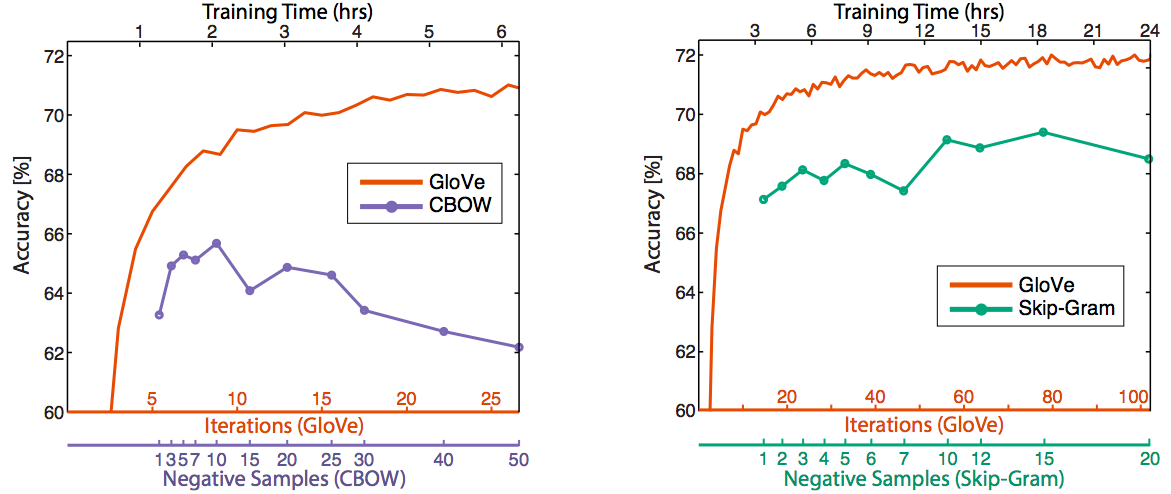
\includegraphics[scale=0.27]{images/gloveVSword2vec.png}
      \caption{From}
    \end{figure}
  \end{figure}
\end{frame}

%%%%%%%%%%%%%%%%%%%%%%%%%%%%%%%%%%%%%%%%%%%%%%%%%%
\begin{frame}{Results}
  \begin{figure}
    \begin{figure}
      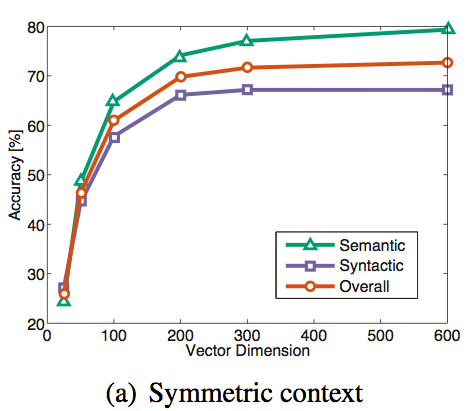
\includegraphics[scale=0.27]{images/analogy1.png}
      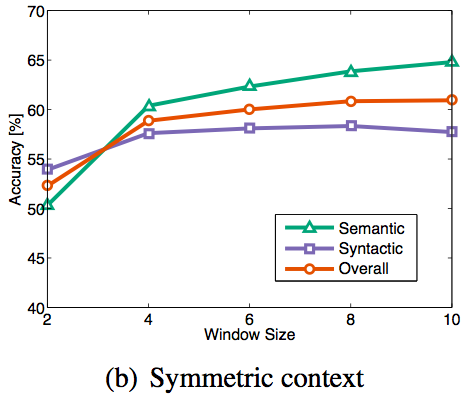
\includegraphics[scale=0.27]{images/analogy2.png}
      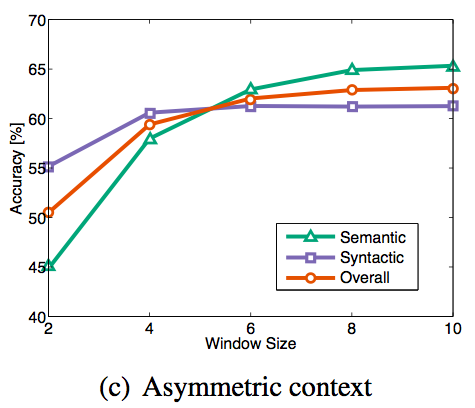
\includegraphics[scale=0.27]{images/analogy3.png}
      \caption{From}
    \end{figure}
  \end{figure}
\end{frame}
